\chapter{Modello Entity Relationship - ER}
In questa parte si studierà la come progettare una base di dati a livello concettuale
e logico, partendo dai requisiti di utente.
Per capirne l'importanza è utile analizzare il ciclo di vita di un sistema informativo
\section{Fasi del ciclo di vita}
\begin{itemize}
    \item Studio di fattibilità: definizione costi e priorità
    \item Raccolta e analisi dei requisiti: studio delle proprietà del sistema
    \item Progettazione: di dati e funzioni
    \item Implementazione: realizzazione
    \item Validazione e collaudo: sperimentazione
    \item Funzionamento: il sistema diventa operativo
\end{itemize}
Il ciclo di vita segue un modello a spirale.
Per garantire prodotti di buona qualità è fondamentale seguire una metodologia
di progetto.
\paragraph*{Metodologia} è un'articolazione in fasi/passi di guida ad una attività di
progettazione.
Avere una metodologia di progetto:
\begin{itemize}
    \item Permette di suddividere la progettazione in fasi
    \item Fornisce una strategia da seguire
    \item Fornisce modelli di riferimento (linguaggi) per descrivere la realtà
    che stiamo progettando
\end{itemize}
Serve per garantire:
\begin{itemize}
    \item Generalità rispetto ai problemi da affrontare
    \item Qualità in termini di correttezza, completezza ed efficienza
    \item Facilità d'uso
\end{itemize}
La metodologia di basa su un principio semplice ma efficace:
\paragraph*{Separazione netta tra decisioni relative a:}
\begin{itemize}
    \item Cosa rappresentare 
    \item Come farlo
\end{itemize}
\section{La progettazione di basi di dati}
La progettazione si divide in 3 fasi:
\begin{itemize}
    \item Progettazione concettuale
    \item Progettazione logica
    \item Progettazione fisica
\end{itemize}
Ognuna delle fasi si basa su un modello, che permette di generare una rappresentazione
formale (schema) della base di dati ad un dato livello di astrazione (concettuale, logico, fisico).
\subsection{Progettazione concettuale}
Traduce i requisiti del sistema informatico in una descrizione formalizzata, integrata
delle esigenze aziendali, espressa in modo \textbf{indipendente} dalle scelte implementative.

\begin{itemize}
    \item Formale - Espressa con un linguaggio non ambiguo e capace di descrivere
    il sistema analizzato
    \item Integrata - Deve essere in grado di descrivere nella globalità l'ambiente analizzato
    \item Indipendete dall'ambiente tecnologico
\end{itemize}
\paragraph*{Nel nostro caso:}
\begin{itemize}
    \item Schema concettuale - \textbf{Modello ER}
    \item Schema logico - \textbf{Modello relazionale}
\end{itemize}
\subsection{Vantaggi della progettazione concettuale}
Permette una descrizione dei dati indipendente dagli aspetti tecnologici con un
livello di astrazione intermedio fra utente e sistema. Prevale l'aspetto intensionale.
\\ Si tratta di una rappresentazione prevalentemente grafica. Utile per la documentazione.
\section{Modello Entità Relazione}
Il modello ER è un modello grafico semi-formale per la rappresentazione di schemi
concettuali. Si è ormai affermato come standard nelle metodologie di progetto e nei
sistemi Software di ausilio alla progettazione.
\section{I Costrutti del modello ER}
\begin{itemize}
    \item Entità
    \item Relazione
    \item Attributo semplice
    \item Atrributo composto
    \item Cardinalità
    \item Cardinalità di un Attributo
    \item Identificatore interno
    \item Identificatore esterno
    \item Generalizzazione
    \item Sottoinsieme
\end{itemize}

\subsection{Entità}
Classe di oggetti (fatti, persone, cose) della applicazione di interesse
con proprità comuni e con esistenza autonoma e della quale si vogliono
registrare fatti specifici.
\begin{center}
    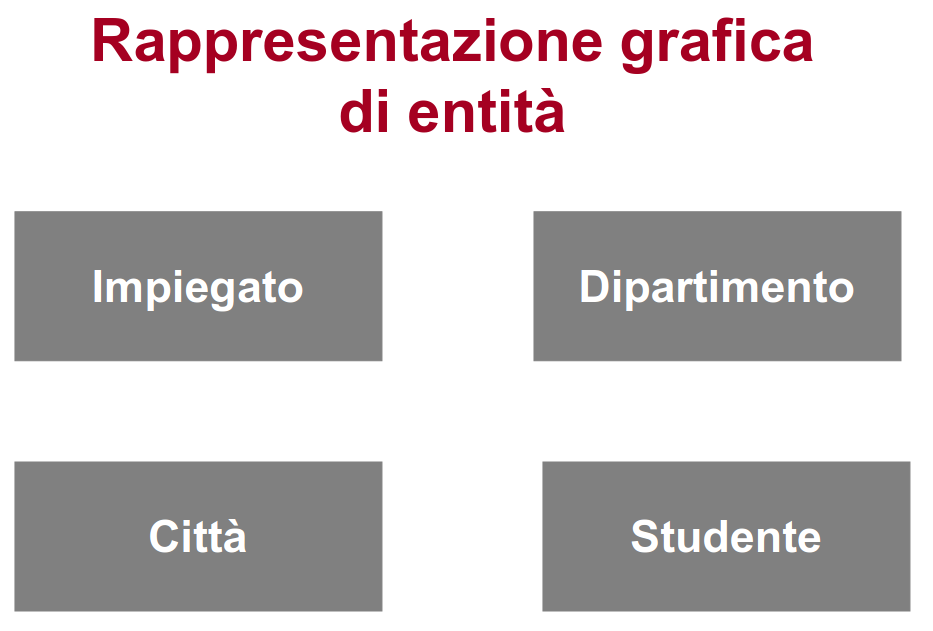
\includegraphics[width=100mm, scale=0.5]{rappresentazione_grafica_entita.png}
\end{center}
Definita come sostantivo al singolare (es. studente, classe, docente, ecc.)
A livello estensionale un'entità è costituira da un insieme di oggetti 
che sono chiamati le sue istanze.
\paragraph*{Istanza}
Occorrenza di un'entità, è l'oggetto della classe che entità rappresenta. Nello schema
concettuale rappresentiamo le entità, non le singole istanze.
\\ Riassumendo:
\begin{itemize}
    \item Conoscenza Astratta $\rightarrow$ Entità
    \item Conoscenza Concreta $\rightarrow$ Istanza di entità
\end{itemize}
\subsection*{Attributi}
Un attributo di un entità è una proprietà locale di un'entità di interesse ai
fini dell'applicazione. Associa ad ogni istanza di un'entità un valore appartenente
a un insieme detto dominio dell'attributo (es. int, string, char, ecc.).
\\ Viene definito quando si vuole rappresentare una proprietà locale
delle istanze dell'entità E.
\\ Una proprietà di un oggetto si dice locale quando in ogni istanza dello schema il valore
di tale proprietà dipende solamente dall'oggetto stesso e non ha alcun rapporto
con altri elementi dell'istanza dello schema.
\paragraph*{Attributi composti}
Si ottengono raggruppando attributi di una medesima entità o relazione che
presentano affinità nel loro significato o uso.
\paragraph*{Esempio:} Indirizzo è composto da Via, Numero, Cap.
\paragraph*{Graficamente} Sono rappresentati come dei collegamenti con un pallino vuoto.
\subsection*{Relazione-Associazione}
Ogni relazione ha un nome che la identifica univocamente nello schema.
\paragraph*{Convenzioni}
\begin{itemize}
    \item Singolare
    \item Sostantivi invece che verbi
\end{itemize}
A livello estensionale una relazione R tra le entità E ed F è costituita da un
insieme di coppie (x, y) tali che x è una istanza di E, ed y è un'istanza di F.
Ogni coppia è detta istanza della relazione R.
\\ Ciò significa che se in uno schema S è definita una relazione R sulle entità E ed F
\paragraph*{Istanze di associazione}
Combinazione (aggregazione) di istanze di entità che prendono parte alla associazione.
\paragraph*{Esempio:} Rossi insegna Basi di Dati
\subsection*{Osservazione importante}
Dalla semantica delle relazioni segue immediatamente che non possono esistere due
istanze della stessa relazione che coinvolgono le stesse istanze di entità.
\\ Due entità possono essere coinvolte in più relationship.
\\ Le relationship possono coinvolgere più di due entità.
\externaldocument[2-Rel]{2-Modello-Relazionale}
\paragraph*{Osservazione sul concetto di relazione} Il concetto di relazione sarà
spiegato meglio nel capitolo 2-Modello-Relazionale.
%Far funzionare link tra 2 diversi file
Una relazione può coinvolgere due o più volte la stessa entità, queste sono
dette \textbf{associazioni ad anello}. In questi casi è fondamentale definire
la specifica dei ruoli, altrimenti non si riesce a capire l'ordine della relazione
(esempio del sovrano o del confronto tra i prof. slide 70-78, 
\href{https://elearning.unimib.it/pluginfile.php/1486876/mod_resource/content/1/Modello%20ER.pdf}{Link}).
\section{Svolgimento Esercizi}
Risulta fondamentale svolgere gli esercizi da casa per allenare la mente a convertire
il testo in schema ER (come sarà all'esame), seguire gli esempi e basta non è sufficiente,
dato che ci saranno diversi dubbi e difficoltà che si faranno strada nella vostra
mente solo se vi metterete a fare gli esercizi per conto vostro (le esercitazioni
sono molto utili).
\section{Scelta tra entità e attributo}
Un dubbio classico nella risoluzione di questi esercizi è proprio la scelta tra
entità e attributo.
\paragraph*{Scelgo Entità quando:}
\begin{itemize}
    \item le sue istanze sono concettualmente significative indipendentemente dalle altre istanze
    \item ha o potrà avere delle proprietà indipendenti dagli altri concetti
    \item se il concetto è importante nell'applicazione
\end{itemize}
\paragraph*{Scelgo Attributo quando:}
\begin{itemize}
    \item le sue istanze non sono concettualmente significative
    \item non ha senso considerare una sua istanza indipendentemente dalle altre
    \item se serve solo a rappresentare un una proprietà locale di un altro concetto
\end{itemize}
\section{Scelta tra entità e relazione}
Dubbio ancora più classico è la scelta tra entità e relazione.
\\ In linea generale quando è necessario modellare un concetto, perchè esiste
a prescindere dalle altre istanze o relazioni allora scelgo entità (es. slide 98).
Oltretutto devo considerare che una relazione esiste in funzione delle sue entità,
viene identificate da una specifica tupla, quindi se ho un caso 
come Studente $\rightarrow$ Esame $\leftarrow$ Corso, dove è possibile che una
persona possa svolgere più volte un esame, questo schema risulta errato dato
che la tupla Studente Corso identifica l'esame e non può identificare più esami svolti 
dalla stessa persona, questo schema quindi impedisce a una persona di dare più esame,
ma come purtroppo sappiamo questo può accadere.
\section{Cardinalità nelle relazioni}
\'E importante definire il numero minimo e massimo di occorrenze delle relazioni cui
ciascuna occorrenza di una entità può partecipare, questo possiamo farlo tramite
la \textbf{cardinalità}.
\\ La cardinalità è una coppia di valori che si associa a ogni entità che partecipa a una
relazione.
\begin{itemize}
    \item 0,1 è la cardinalità minima \begin{itemize}
        \item 0 = partecipazione opzionale
        \item 1 = partezipazione obbligatoria
    \end{itemize}
    \item 1 e N per la massima - N non pone alcun limite
\end{itemize}
\paragraph*{Esempio:} Slide 105, cardinalità Residenza dove una città ha più residenze,
mentre uno studente ne ha una sola.
\\ Per quanto riguarda le cardinalità massime, abbiamo relazioni
\begin{itemize}
    \item 1,1 se la cardinalità massima di entrambe le entità è 1
    \item Si può avere 1 a molti come nell'esempio della residenza
    \item Oppure sei può avere molti a molti (slide 108 riporta esempi)
\end{itemize}
\subsection*{Praticità della cardinalità}
A livello pratico la cardinalità esprime un limite mino (cardinalità minima)
e massimo (cardinalità massima) di istanze della relazione R a cui può partecipare
ogni istanza dell'entità E. Serve a caratterizzare meglio il significato di una relazione.
\paragraph*{Attributi e cardinalità} Si può assegnare cardinalità anche agli attributi
per indicare opzionalità o attributi multivalore.
\section{Identificatore di un'entità}
Super importante è definire un identificatore per ogni entità, necesasrio per identificare
univocamente le occorrenze di un'entità.
\begin{itemize}
    \item \textbf{Identificatore interno} - se costituito da attributi dell'entità
    \item \textbf{Identificatore esterno} - attributi + entità esterne attraverso relationship
\end{itemize}
\subsection*{Notazione identificatori}
Per gli identificatori interni:
\begin{itemize}
    \item Se l'identificatore è costituito da un solo attributo, si annerisce il corrispondente
    pallino
    \item Se l'identificatore è costituito da più attributi, si uniscono gli attributi con
    una linea che termina con un pallino annerito
\end{itemize}
Per gli identificatori esterni:
\begin{itemize}
    \item Se l'identificatore è formato da attributi e relazioni (o meglio ruoli) si
    indica unendo gli attributi ed i ruoli con una linea che termina con un pallino annerito
\end{itemize}
\subsection*{Osservazioni}
\begin{itemize}
    \item Ogni entità deve possedere almeno un identificatore, ma può averne in generale più di uno.
    \item \textbf{Una identificazione esterna è possibile solo attraverso una relationship a
    cui l'entità da identificatore partecipa con cardinalità (1,1)}
    \item In questo corso \textbf{NON si utilizzano identificatori delle relationship}
\end{itemize}
\section{Relazione IS-A tra entità}
\'E una relazione di sottoinsieme di un entità, si può definire come entità-padre
ed entità figlia, o sottoentità, cioè quella che rappresenta un sottoinsieme della
entità padre.
\paragraph*{Esempio}Persona $\rightarrow$ Studente, dove Studente è una sottoentità
di Persona. Si dice che Studente è in relazione ISA con Persona o in alternativa
che Studente ISA Persona.
Si tratta di un sottoinsieme specifico di quell'entità, esso eredita tutte le
proprietà del padrea, quindi i suoi attributi (non vengono riportati nel figlio, ma sono
presenti), ciò non toglie che il figlio possa avere attributi aggiuntivi.
\paragraph*{Ereditarietà} Tutte le proprietà (attributi, relationship, altre generalizzaizoni)
dell'entità genitore vengono ereditate dalle entità figlie e non rappresentate
esplicitamente.
\section{Generalizzazione tra Entità}
Nella relazione ISA l'entità padre è più generale della sottoentità. Talvolta
l'entità padre può generalizzare diverse sottoentità rispetto ad un unico
criterio. In questo caso si parla di \textbf{generalizzazione}.
Nella generalizzazione le sottoentità hanno insiemi di istanze disgiunti a coppie.
\\ Una generalizzazione può essere di due tipi:
\begin{itemize}
    \item Completa - L'unione delle istanze delle sottoentità è uguale all'insieme
    delle istanze dell'entità padre
    \item Non completa
\end{itemize}
\paragraph*{Graficamente} La generalizzazione si indica collegando
mediante un arco le sottoentità e collegando con una freccia tale arco alle entità
padre. La freccia è annerita solo se la generalizzazione è completa.
\paragraph*{Esempio} Persona $\rightarrow$ Uomo/Donna (generalizzazione completa)
\paragraph*{Esempio} Persona $\rightarrow$ Studente/Docente (generalizzazione non completa)
\paragraph*{Regola importante} Vige la regola che una entità può avere al massimo
una entità padre. In altre parola, il modello ER \textbf{NON ammette ereditarietà multipla}.
Sia per quanto riguarda le ISA e le generalizzazioni.
\\ Mentre la stessa entità può essere padre di diverse generalizzazioni.
\paragraph*{Ereditarietà} Anche in questo caso vale il principio di ereditarietà.
\subsection*{Differenze tra due IS-A e una generalizzazione}
Le due sottoclassi della generalizzazione derivano da uno stesso criterio di
classificazione della superclasse, mentre per quanto riguarda la relazione IS-A
le due sottoentità sono indipendenti.

